


\documentclass[a4paper]{article}
\usepackage{graphicx, fullpage, float, subfig, verbatim,amsmath, multirow, fancyhdr, hyperref}
\usepackage[utf8]{inputenc} 
\usepackage[norsk]{babel}
\usepackage{empheq}
\usepackage[dvipsnames,table]{xcolor}
\definecolor{medGray}{RGB}{230,230,230}

\newenvironment{important}[2][]{
        \setkeys{EmphEqEnv}{#2}
        \setkeys{EmphEqOpt}{box={\setlength{\fboxsep}{10pt}\colorbox{medGray}},#1}
        \EmphEqMainEnv}
{\endEmphEqMainEnv}

\title{\textbf{''Gisse GIS''  \\- webbasert geografisk informasjonssytem ved hjelp av Open Source-programvare}
\\ \normalsize TBA 4251 - Programmering i geomatikk, høsten 2012}
\author{Steffen Pøhner Henriksen}
\date{\today}

\begin{document}
\maketitle
\vspace{3cm}

\pagebreak

\begin{abstract}

	Gisse GIS er resultatet av min innsats i faget "TBA4251 - Programmering i geomatikk". Det er et enkelt geografisk informasjonssystem som kjører i en nettleser. Ved hjelp av Open Source-programvare vises vektordata over fritt tilgjenglige bakgrunnskart. Vektordataene kan så manipuleres med metoder kjent fra kraftfulle GIS som er desktop-applikasjoner. Metodene som støttes i dag er:
	
	\begin{itemize}
		\item Buffer - Utvider valgt område med en gitt verdi i meter.
		\item Area - Gir arealet av området i kvadratmeter.
		\item Merge - Slår sammen to vektorlag.
		\item Subtract - Trekker et vektorlag fra et annet.
		\item Intersect - Returnerer overlappende vektorlag.
		\item Distance - Finner minste avstand mellom to vektorlag.
		\item Simplify - Forenkler geometrien til et vektorlag ved Douglas-Peuker. 
	\end{itemize}
	
	Programmet består av tre deler - database, serverlag og klient. Kommunikasjonen mellom server og klient skjer via Websockets\cite{websockets}. Klienten er skrevet i Javascript, med HTML5 og CSS3. Tilleggsbiblioteker som er brukt i klienten er Knockout.js og jQuery, samt Twitter Bootstrap. Serverlaget er skrevet i node.js som tilbyr Javascript til bruk for serverkode. Her er sockets.io, Express og databasedriver brukt som tilleggsbiblioteker. Eksempeldata brukt i utviklingen og til demostrasjon er hentet fra Open Street Map og lagres i en PostgreSQL-database med PostGIS-utvidelse. Alt er lagret i skyen hos Amazons EC2-tjeneste, som sørger for at programmet leveres til brukers nettleser. 
	
	Resultatet er et brukervennlig GIS som utfører enkle operasjoner vi kjenner fra før, på frie vektordata som eksempel. ''Gisse GIS'' kan prøves ved å besøke adressen http://gisse.pohnerhenriksen.com i din nettleser.
	
\end{abstract}
\newpage

\tableofcontents
\newpage

\section{Innledning}
	
	Denne rapporten omhandler arbeidet med ''Gisse GIS'' utført høsten 2012. Den er et resultat av faget ''TBA4251 - Programmering i Geomatikk'' ved NTNU. Denne rapporten argumenterer for valg av programmeringsspråk, tilleggsbiblioteker og fremgangsmåte i arbeidsprosessen. Dataflyt og strukturen av programmet blir lagt frem. Et forslag til et scenario for å teste programmet blir også presentert. Oppdagede bugs, feil og mangler blir listet opp og kommentert. 
	
	Man kan dele inn arbeidet i fire deler - design, implementering, bugfiksing og rapportskriving. En stor del av arbeidet med utarbeidelsen av programmet var definere hva det skulle bli, hvilke verktøy som var hensiktsmessig å bruke, samt lære seg disse verktøyene. Tidlig ble det bestemt at jeg ville velge GIS-oppgaven i faget. Det gav meg muligheten til å jobbe med Javascript/HTML, noe jeg ikke har brukt i noen særlig grad før og har lyst til å lære meg. Oppgaven er farget av at jeg i størst mulig grad ville benytte meg av Open Source-programvare, og gjøre meg kjent med hva som finnes av slik programvare for bruk i geomatikkfaget. 
	
	\begin{quotation}
		"Software is like sex: it's better when it's free." 
			\em  -- Linus Torvalds
	\end{quotation}
	
	Tidligere har jeg jobbet hos Norkart AS som systemutvikler. Her laget jeg en database/server-løsning som behandlet geografiske data med tilleggsinformasjon. Kunnskapen fra denne sommerjobben kom godt med i utarbeidelsen av oppgaven. Kunnskapen opparbeidet herfra gjorde at jeg raskt så muligheter som PostGIS gir, og at implementeringen av databasedelen gikk relativt lett.
	
	
	
	\begin{figure}[h]
	\centering
	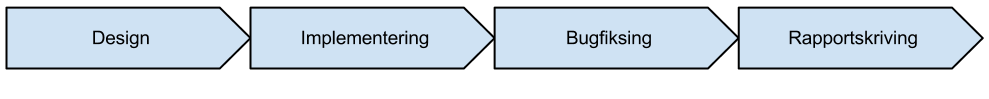
\includegraphics[scale=0.5]{innledning.png}
	\caption{Arbeidsprosess}
	\end{figure}
	
\section{Formål med applikasjonen}

\section{Valg av programmeringsspråk}
	
	\subsection{HTML5 og CSS3}
		\subsubsection{Twitter Bootstrap}
		\subsubsection{Leaflet}
	\subsection{JavaScript}
		\subsubsection{jQuery}
		\subsubsection{Knockout.js}
		\subsubsection{Node.js}
		\subsubsection{socket.io}
	\subsection{PostgreSQL - PostGIS}

\section{Server i skyen - Amazon EC2}

\section{Testscenario}
\section{Bugs, feil og mangler}
	\subsection{Forbedringspotensiale}
\section{Diskusjon - Løser applikasjonen oppgaven?}

\newpage
\begin{thebibliography}{9}

\bibitem{websockets}
	Wikipedia: Websockets, http://en.wikipedia.org/wiki/WebSocket, 22.12.2012


\end{thebibliography}

\end{document}

